\chapter{Proposta para análise de arquiteturas \ac{mmorpg}}
\label{cap3}



As arquiteturas de serviços \ac{mmorpg} são desenvolvidas visando suprir as necessidades do \textit{design} do jogo desenvolvido, de forma a qual viabilize o comércio deste serviço como produto.
%
Nesse sentido, jogos com mecânicas de \textit{design} parecidos possuem implementações parecidas para os clientes.
%
Entretanto, a arquitetura escolhida impacta no custo de operação e qualidade do serviço aos jogadores.
%
Por este motivo, diferentes arquiteturas com o mesmo \textit{design} não são comparáveis entre sí, visto que dependem das regras de negócio.



Ao desenvolver um serviço \ac{mmorpg} é necessário decidir uma arquitetura a qual reduza custos, consumo de recursos e minimize ocorrências para os jogadores a fim de viabilizar o seu comércio como produto.
%
Porém, a impossibilidade de comparação direta entre as arquiteturas de serviço \ac{mmorpg} instiga a análise das características básicas que possam influenciar o \textit{game design}, tais como consumo de recursos, tempo de resposta, latência e número máximo de clientes.
%
Sendo assim, uma analise do consumo de recursos computacionais das arquiteturas levantadas previamente na literatura tem valor científico no auxílio na escolha de implementações arquiteturas de microsserviços, em específico para serviços \ac{mmorpg}.



Nesta seção é descrito a proposta para análise de consumo de recursos computacionais em arquiteturas \ac{mmorpg}.
%
A atual seção descreve a Proposta (Subseção~\ref{sec:proposta}), trazendo os objetivos desta análise, quais recursos e métricas serão analisadas.
%
Os Critérios de Análise (Subseção~\ref{sec:criterios}) exibem como os dados obtidos devem ser interpretados, baseando-se nos objetivos da análise das arquiteturas.
%
O Plano de Testes (Subseção~\ref{sec:plano}) exibe como será realizada a coleta dos dados, descrevendo cenários, critérios e objetivos dos testes.



\section{Proposta}
\label{sec:proposta}

Tendo analisado os trabalhos relacionados e as arquiteturas específicas para jogos \ac{mmorpg}, o presente trabalho tem como objetivo analisar as arquiteturas \ac{mmorpg} visando complementar os recursos computacionais não analisados nos trabalhos relacionados.
%
Em específico, serão obtidos das arquiteturas Rudy (Subseção~\ref{rudy}), Salz (Subseção~\ref{salz}) e Willson (Subseção~\ref{willson}) os seguintes valores referente aos recursos (Tabela~\ref{tab:recursos_categoria}):

\begin{enumerate}
  \item \ac{cpu};
  \item Memória;
  \item Banda.
\end{enumerate}

Além dos recursos computacionais, esta análise levará em conta valores referente a outras métricas.
%
As métricas, cujos os valores serão obtidos são:

\begin{enumerate}
  \item Limite de conexões;
  \item Tempo de resposta;
  \item Latência.
\end{enumerate}

Para prever o comportamento destas métricas e recursos, serão calculadas as complexidades das operações usadas no plano de teste.
%
Espera-se em situações adversas, caracterizar os comportamentos, gargalos e o custos computacionais para manutenção dos serviços em cada arquitetura.
%
Para este fim, se faz necessário a descrição dos critérios que serão utilizados durante a análise dos valores obtidos nos experimentos.

%ccm
% objetivos
% Definição das métricas para os itens levantados nas Tabelas 2.4 e 2.5

\section{Critérios de análise}
\label{sec:criterios}

A fim de realizar a análise das arquiteturas de microsserviços específicos a jogos \ac{mmorpg}, se faz necessário definir critérios para analisar os valores obtidos.
%
Os critérios de análise vão guiar os casos de teste e a análise das arquiteturas.

O uso de \ac{cpu} está relacionado com os algoritmos empregados no serviço.

O uso de memória deve estar relacionado diretamente ao número de jogadores simultâneos no serviço.

O uso de banda está relacionado a complexidade da arquitetura de microsserviços e número de conexões necessários para manter a comunicação com o serviço.

O limite de conexões está relacionado escalabilidade dos serviços e o consumo do gerenciamento da arquitetura.

O tempo de resposta está relacionado diretamente ao número de conexões a um microsserviço e ao modelo de processamento de chamadas remotas.

A latência poderá trazer informações sobre o meio físico entre os clientes e o serviço.

Espera-se relacionar as informações obtidas a fim de obter características das arquiteturas de microsserviços.

\begin{itemize}
  \item Tabelas de consumo de recurso por cenário;
  \item Gráficos de relação de consumo de recursos por número de conexões;
\end{itemize}




%ccm
% Identificar como os valores obtidos pelas métricas devem ser interpretados
% pode ser individdual ou em grupos, defiir a finalidade? Custo? Desempenho?

%ccm Usar os critérios das colunas das Tabelas 2.4 e 2.5 de modo a deixar clara a importância de realizar uma análise que contemple todos os itens e não apenas partes deles, como identificado nos trabalahos relacionados (Seção 2.7).

\section {Plano de testes}
\label{sec:plano}

O plano de testes definirá os cenários que serão aplicados sobre todas as arquiteturas de microsserviços para jogos \ac{mmorpg}.
%
Ele servirá para descrever formas de estressar as arquiteturas, a fim de obter os valores para análise.
%
Os cenários existentes são:



\begin{enumerate}
  \item \textbf{Cenário I}: Um único jogador durante um tempo determinado;
  \item \textbf{Cenário II}: Crescimento linear de jogadores simultâneos até exceder o limite de conexões da arquitetura;
  \item \textbf{Cenário III}: Número de jogadores simultâneos a partir de uma amostra obtida de um ambiente real;
\end{enumerate}



No \textbf{Cenário I}, espera-se obter métricas fixas do funcionamento básico do serviço.
%
Desta forma, espera-se obter características para serviços com um número de jogadores simultâneos baixo, caracterizando o mínimo de recurso utilizado pela arquitetura.



No \textbf{Cenário II}, espera-se estressar o serviço para obter métricas em um linear crescente de jogadores simultâneos, até ele exceder o limite de conexões da arquitetura.
%
Neste cenário espera-se encontrar tanto o limite de conexões simultâneas e suas características por número de conexões.
%
Com este cenário planeja-se estressar todos os recursos, e será um cenário propício para obter métricas relevantes sobre gargalos dos algoritmos implementados, consumo de banda e tempo de resposta.



No \textbf{Cenário III}, espera-se obter métricas referente a uma utilização real de um serviço \ac{mmorpg}.
%
Desta forma, espera-se obter uma situação aproximada de uma arquitetura em ambiente de produção.
%
É planejado que este cenário gere dados com valores distintos de conexões, e por este motivo diversifiquem os dados obtidos a fim de gerar maior confiabilidade nas conclusões da análise.


A infraestrutura planejada para os testes será dividida em cinco camadas:
\begin{enumerate}
  \item \textbf{Serviço de Jogo}: A camada de serviço da infraestrutura dos testes concentrará a arquitetura de microsserviços referente as arquiteturas de microsserviços analisadas.
  \item \textbf{Banco de dados do serviço de jogo}: A camada de banco de dados do serviço de jogo conterá os serviços de dados e web a fim de manter um padrão de dados no serviço \ac{mmorpg}.
  \item \textbf{Estresse}: A camada de estresse será responsável por realizar requisições ao serviço a fim de estressá-lo.
  \item \textbf{Cliente}: A camada de cliente será composta pelos mesmos elementos da camada de estresse, porém em um ambiente controlado para que a suíte de stress não interfira nas métricas obtidas no lado do cliente.
  \item \textbf{Dados}: A camada de dados será composta por algum banco de dados de log a fim de armazenar os dados obtidos da camada Cliente.
\end{enumerate}

Esta separação se faz importante para que demais camadas não interfiram nos valores obtidos.
%
A camada de banco de dados do serviço de jogo, estresse, cliente e dados serão fixos a fim de reduzir alterações nos valores obtidos por conta de implementações diferentes.
%
O serviço de banco de dados do serviço de jogo e serviço de jogo será alterado conforme o caso de uso sobre as arquiteturas descritas na referenciação teórica.
%
O plano de testes será executado sobre a infraestrutura na qual pode ser visualizada na Figura~\ref{infraestrutura}.

\begin{figure}[htb!]
  \caption{Infraestrutura definida para os cenários de teste}
  \label{infraestrutura}
  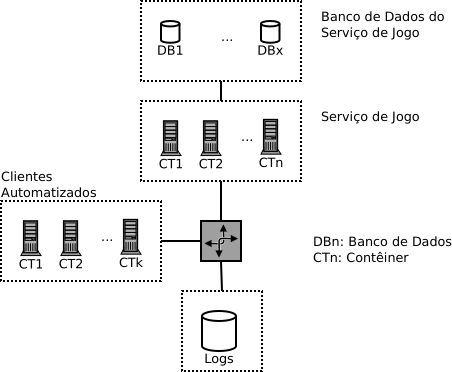
\includegraphics[height=6.5cm]{img/cap3/infraestrutura.png}
  \centering

  Fonte: O próprio autor.
\end{figure}

A infraestrutura definida na Figura~\ref{infraestrutura} será elaborada na nuvem de computadores do \ac{labp2d}, a qual opera sobre o sistema OpenStack\footnote{OpenStack: \url{https://www.openstack.org/}}, facilitando assim a criação desta infraestrutura virtual.

A execução dos cenários ocorrerão utilizando as arquiteturas Rudy (~\ref{rudy}), Salz (~\ref{salz}) e Willson(~\ref{willson}), sendo referenciados no atual trabalho como casos de uso.
%


%ccm Genérico/abstratpo
% Quais experimentos serão realizados, se não necessário explicitar os caso de uso e o quê espera-se de resultado.
% 
% Descrever como cenários, critérios e objetivos de testes.
